\documentclass[preprint,12pt]{elsarticle}
\usepackage{amsmath,amssymb}
\usepackage{graphicx}
\usepackage{booktabs}
\usepackage{siunitx}
\usepackage{lineno}
\usepackage[hidelinks]{hyperref}
\usepackage{xcolor}
\graphicspath{{figures/}}
\newcommand{\betaErr}{1.9}
\newcommand{\aeffFD}{5.28}
\newcommand{\aeffDiff}{2.1}
\newcommand{\lamg}{9.91}
\newcommand{\STLtl}{-0.24}
\newcommand{\Kfit}{17.2}
\newcommand{\Lres}{3.8}
\newcommand{\LresIso}{4.12}
\newcommand{\gslot}{0.20}
\newcommand{\gsum}{1.08}
\newcommand{\SSum}{0.04}
\newcommand{\fAir}{33.3}
\newcommand{\epsEff}{1.88}
\newcommand{\Ld}{3.96}
\newcommand{\BWref}{28.20--28.43}
\newcommand{\BWrefRel}{0.8}
\newcommand{\BWdec}{28.23--28.68}
\newcommand{\fcDec}{28.5}
\newcommand{\BWdecRel}{1.6}
\newcommand{\BWsixRef}{27.55--29.05}
\newcommand{\BWsixDec}{27.77--29.07}
\newcommand{\BWsixDecRel}{4.6}
\newcommand{\SElevenDec}{-11.3}
\newcommand{\SElevenRef}{-10.4}
\newcommand{\IsoRefTwentyEight}{-17.5}
\newcommand{\IsoDecTwentyEight}{-23.5}
\newcommand{\IsoRefMin}{-17.2}
\newcommand{\IsoDecMin}{-20.5}
\newcommand{\IsoGain}{5.9}
\newcommand{\IsoSeventy}{-15.3}
\newcommand{\IsoSeventyMin}{-14.9}
\newcommand{\BWseventy}{28.15--28.73}
\newcommand{\GainSeventy}{10.9}
\newcommand{\Dfin}{9.4}
\newcommand{\Lduse}{4.0}
\newcommand{\Xoff}{0.8}
\newcommand{\IsoDecMax}{-26.2}
\newcommand{\GainRef}{10.1}
\newcommand{\GainDec}{11.9}
\newcommand{\EffDec}{96}
\newcommand{\GainDelta}{1.8}
\newcommand{\HPBWe}{23}
\newcommand{\HPBWh}{62}
\newcommand{\TiltRef}{+13}
\newcommand{\TiltDec}{+7}
\newcommand{\ECCref}{0.014}
\newcommand{\ECCdec}{0.033}
\newcommand{\CondLoss}{0.11}
\newcommand{\MSref}{1.00}
\newcommand{\GCIref}{1.17}
\newcommand{\GCIslit}{0.36}
\newcommand{\platesize}{15.6~mm$\times$~29~mm}
\newcommand{\SweepSentence}{see Table~\ref{tab:sweep}}

\journal{AEU -- Int. J. Electron. Commun.}

\begin{document}
\begin{frontmatter}

\title{Low-profile SIW slot array with characteristic-mode-guided decoupling for 28~GHz 5G mmWave front ends: an open-source hybrid FDTD/MoM design environment}

\author[vcet]{M.~Nisha Angeline\corref{cor1}}
\ead{nishavlsidesign@gmail.com}
\cortext[cor1]{Corresponding author.}
\affiliation[vcet]{organization={Department of Electronics and Communication Engineering, Velalar College of Engineering and Technology},
  city={Thindal, Erode}, state={Tamil Nadu}, country={India}}

\begin{abstract}
A low-profile, dual-port substrate-integrated-waveguide (SIW) longitudinal-slot array for the 28~GHz 5G mmWave band (n257/n261) is designed, and the mutual coupling between its two closely spaced $1\times5$ sub-arrays is suppressed with resonant slits etched in the common top wall whose length is dimensioned by characteristic-mode analysis (CMA). The complete design is carried out in an open-source environment written for this work: a Numba-accelerated three-dimensional finite-difference time-domain (FDTD) solver on a nonuniform Yee grid with convolutional perfectly matched layers and TE$_{10}$ waveguide ports, a Rao--Wilton--Glisson method-of-moments (MoM) solver with a Harrington--Mautz characteristic-mode eigensolver in both the electric-current (finite plate) and magnetic-current (aperture) formulations, and the classical SIW/Elliott synthesis equations. The FDTD solver reproduces the analytical SIW TE$_{10}$ dispersion within \betaErr\,\% at 28~GHz. Full-wave single-slot characterisation on the \SI{0.508}{mm} RT/duroid~5880 substrate shows that the resonant conductance follows $g = K\sin^2(\pi x_0/a)$ with $K = \Kfit$, an order of magnitude above the thick-waveguide Stegen value, so that a five-slot standing-wave sub-array is matched with offsets of only \SI{0.2}{mm}. The two sub-arrays are spaced $D = \SI{7}{mm}$ ($0.65\lambda_0$) apart and exhibit a port isolation of only \IsoRefTwentyEight~dB at 28~GHz. CMA of the aperture system and of the finite top wall identifies the gap-crossing current mode responsible for the coupling and yields a slit length of \Ld~mm for a 28~GHz characteristic resonance; the FDTD verification confirms an isolation improvement to \IsoDecTwentyEight~dB at 28~GHz (\IsoGain~dB improvement) and a minimum in-band isolation of \IsoDecMin~dB over the \BWdec~GHz common $-10$~dB band, with a realised gain of \GainDec~dBi, an envelope correlation coefficient below \ECCdec and a total thickness of \SI{0.58}{mm} ($0.054\lambda_0$). All solvers, scripts and data are released, making the design reproducible without commercial electromagnetic software.
\end{abstract}

\begin{keyword}
substrate integrated waveguide \sep slot array \sep characteristic modes \sep mutual coupling \sep decoupling \sep 28~GHz \sep 5G mmWave \sep FDTD \sep method of moments \sep open-source
\end{keyword}
\end{frontmatter}

\linenumbers

\section{Introduction}
Millimetre-wave (mmWave) bands around 28~GHz are central to 5G New Radio because of the contiguous spectrum they offer, but the free-space path loss and the blockage sensitivity of these bands require directive, electronically steerable antennas at both the base station and the user terminal \cite{rappaport2013,hong2017}. The front-end antenna must therefore be a compact array that is thin enough to be embedded in a handset or in a tile of a massive-MIMO panel, that integrates with the printed-circuit-board (PCB) feed of the transceiver, and that offers sufficient port-to-port isolation for the sub-arrays to be driven independently \cite{yang2017tsa,zhang2023wideband}.

Substrate integrated waveguide (SIW) technology provides exactly this combination of low profile, low loss and PCB compatibility at mmWave frequencies \cite{deslandes2006,xu2005,cassivi2002,coves2021}. Longitudinal-slot arrays cut in the broad wall of an SIW are the planar counterpart of the classical waveguide slot arrays and can be synthesised with Elliott's procedure once the admittance of an isolated slot is known \cite{elliott1983,elliott2003,yang2014,yang2015conformal,mallahzadeh2015}. Several SIW slot arrays have been reported for the 28~GHz band \cite{ashraf2015,lai2020,sun2020qmsiw,singh2021,kobal2022}, usually as single-port arrays fed by a corporate SIW divider. When two or more SIW sub-arrays are placed side by side on the same substrate, however, their slots share one continuous top metal, and the strong E-plane coupling between parallel slots leads to a port isolation of only 15--20~dB for a centre spacing of $0.6$--$0.7\lambda_0$, which degrades the active reflection coefficient, the beam-scanning range and the diversity performance of the front end. Reported remedies include metamaterial or electromagnetic-bandgap shields \cite{alibakhshikenari2019,dey2021}, indirect-coupling feed networks \cite{diman2021}, via chokes and field-confining structures \cite{zhang2023wideband}. These solutions are either bulky (additional layers or periodic cells) or specific to one feed topology.

The theory of characteristic modes (TCM) \cite{harrington1971,harrington1971b,cabedo2007,chen2015,ylaoijala2019} has recently become a systematic tool for decoupling, because the eigencurrents of the shared conductor reveal which mode carries energy from one port to the other and how the structure must be perturbed to suppress it \cite{lai2023self,sun2021cmdm,fritz2020,cao2022,qu2023,chen2024lc}. Most of these works address sub-6~GHz terminal antennas on finite ground planes; the application of TCM to the shared top wall of SIW slot arrays at mmWave frequencies has, to the best of our knowledge, not been reported.

A second practical obstacle is that the design of such structures is normally tied to commercial full-wave software, so that the published results cannot be reproduced or extended by groups without access to those licences. This paper addresses both issues. Its contributions are:
\begin{enumerate}
\item an open-source electromagnetic design environment, written from scratch in Python with Numba acceleration \cite{lam2015numba}, comprising a 3-D FDTD solver \cite{taflove2005,roden2000} with SIW waveguide ports and an aperture near-to-far-field transformation, an RWG method-of-moments solver \cite{rwg1982} with a characteristic-mode eigensolver in both the electric-current and the magnetic-current (aperture) formulation, and the analytical SIW and slot-array synthesis equations; the solvers are validated against the analytical SIW dispersion relation and the resonance of a strip dipole;
\item the full-wave characterisation of a longitudinal slot in a thin ($h = 0.047\lambda_0$) SIW at 28~GHz, showing that the resonant conductance per slot is an order of magnitude larger than predicted by the Stegen formula and that the slot resonance shifts strongly with the offset, and the resulting Elliott synthesis of a $1\times5$ standing-wave sub-array with 0.2~mm offsets;
\item a characteristic-mode-guided decoupling method in which resonant slits etched in the common top wall between the sub-arrays are dimensioned from the aperture-mode resonance and verified on the finite top wall through the modal significance and the gap-crossing current of the coupling mode, giving a \IsoGain~dB improvement of the 28~GHz isolation at no cost in profile, footprint or gain.
\end{enumerate}
Section~\ref{sec:env} describes the design environment and its validation, Section~\ref{sec:design} the sub-array synthesis, Section~\ref{sec:cma} the characteristic-mode analysis and the slit design, Section~\ref{sec:results} the full-wave results and a comparison with the literature, and Section~\ref{sec:concl} the conclusions.

\section{Open-source design environment}\label{sec:env}
\subsection{Architecture}
The environment (\texttt{siwlab}, released with this paper) is organised in five modules. \texttt{siw} implements the equivalent-width, cutoff, dispersion and attenuation relations of the SIW; \texttt{slots} implements the Elliott standing-wave synthesis with full-wave slot data; \texttt{mesh} and \texttt{mom} implement the triangular mesher, the RWG electric-field integral equation (EFIE), its magnetic-current dual for apertures in a ground plane, and the characteristic-mode eigensolver; \texttt{fdtd} and \texttt{geometry} implement the 3-D FDTD solver and the parametric SIW array builder. All computations reported here were run on four CPU cores; the longest single FDTD run takes about ten minutes.

\subsection{SIW model}
For via diameter $d$, pitch $p$ and via-row spacing $a$ the equivalent rectangular-waveguide width is $a_{\mathrm{eff}} = a - d^2/(0.95p)$ \cite{cassivi2002}, and the TE$_{10}$ phase constant is $\beta = \sqrt{k_0^2\varepsilon_r - (\pi/a_{\mathrm{eff}})^2}$. The design rules $p \le 2d$ and $d < \lambda_c/5$ \cite{deslandes2006,xu2005} are checked automatically. The substrate is Rogers RT/duroid~5880 ($\varepsilon_r = 2.2$, $\tan\delta = 0.0009$, $h = \SI{0.508}{mm}$) with $d = \SI{0.4}{mm}$, $p = \SI{0.8}{mm}$ and $a = \SI{5.6}{mm}$, giving $a_{\mathrm{eff}} = \SI{5.39}{mm}$ and $f_c = \SI{18.75}{GHz}$, i.e. $f_c/f_0 = 0.67$ at 28~GHz.

\subsection{FDTD solver}
The FDTD solver uses a nonuniform Yee grid (\SI{0.1}{mm} cells in the SIW and slot region, graded to \SI{0.2}{mm} in the margins and to \SI{0.25}{mm} in the air above the array; five cells across the substrate), convolutional PML (CPML) \cite{roden2000} on the lateral and upper boundaries, a perfect electric conductor (PEC) on the lower boundary (ground plane), cell-averaged permittivity and conductivity on the field edges, and edge-based PEC masks for the top metal, the vias (cell-centred staircase that conserves the via cross-section) and the shorting walls. The via rows are extended into the PML so that the SIW feed lines are matched. A TE$_{10}$ mode is launched as a soft $E_z$ source with the profile $\sin[\pi(x-x_1)/a_{\mathrm{eff}}]$ and the modal voltage and current, $V(t) = \iint E_z\,s\,\mathrm{d}S$ and $I(t) = \iint H_x\,s\,\mathrm{d}S$, are recorded on reference planes. The S-parameters follow from the ratio of the spectra to those of a slot-free reference line with identical source and grid, which also yields the incident power $P_{\mathrm{inc}} = \mathrm{Re}(VI^\ast)/(2N)$ with $N = \iint s^2\,\mathrm{d}S$. The tangential field in every aperture of the top wall is accumulated by a running discrete Fourier transform, and the far field is obtained from the equivalent magnetic current $\mathbf{M} = -2\hat{\mathbf{z}}\times\mathbf{E}_a$ on the infinite PEC plane \cite{balanis2016}; the radiated power from the hemisphere integral of the radiation intensity gives the radiation efficiency, and the envelope correlation coefficient (ECC) is computed from the embedded far fields of the two ports \cite{blanch2003}. The excitation is a Gaussian-modulated pulse centred at 28~GHz with a 1/e half-bandwidth of 6~GHz; the time step is $\Delta t = \SI{0.1885}{ps}$ (Courant number 0.99) and the simulated interval is 2.6~ns for the single-slot and 3.6~ns for the array models. Numba just-in-time compilation with parallel loops gives \SI{10}{ms} per time step for $2.3\times10^6$ cells.

\subsection{MoM and characteristic-mode solver}
The EFIE is discretised with RWG basis functions on a structured triangular mesh whose lines coincide with every aperture edge. The impedance matrix
\begin{equation}
Z_{mn} = \mathrm{j}\omega\mu\iint \mathbf{f}_m\cdot\mathbf{f}_n G\,\mathrm{d}S\,\mathrm{d}S' - \frac{1}{\mathrm{j}\omega\varepsilon}\iint (\nabla\!\cdot\!\mathbf{f}_m)(\nabla\!\cdot\!\mathbf{f}_n) G\,\mathrm{d}S\,\mathrm{d}S'
\label{eq:zmn}
\end{equation}
is assembled triangle-pair-wise with a six-point Gauss rule on the test triangle and a $4^4$ ($4^5$ for the self term) barycentric subdivision of the source triangle for near interactions, in parallel Numba kernels. The characteristic modes are the solutions of $\mathbf{X}\mathbf{J}_n = \lambda_n\mathbf{R}\mathbf{J}_n$ \cite{harrington1971b}, computed after projecting onto the subspace of $\mathbf{R}$ with eigenvalues above $10^{-9}$ of its maximum, and tracked over frequency by the $\mathbf{R}$-weighted correlation of the eigencurrents. The modal significance is $\mathrm{MS}_n = |1+\mathrm{j}\lambda_n|^{-1}$ and the characteristic angle $\alpha_n = 180^\circ - \arctan\lambda_n$ \cite{cabedo2007}. For apertures in an infinite ground plane the dual (magnetic-current) formulation is used: with the image theorem the aperture admittance operator of each half-space $i$ is
\begin{equation}
Y^{(i)}_{mn} = 2\Big[\mathrm{j}\omega\varepsilon_i\iint \mathbf{f}_m\cdot\mathbf{f}_n G_i\,\mathrm{d}S\,\mathrm{d}S' - \frac{1}{\mathrm{j}\omega\mu_0}\iint (\nabla\!\cdot\!\mathbf{f}_m)(\nabla\!\cdot\!\mathbf{f}_n) G_i\,\mathrm{d}S\,\mathrm{d}S'\Big],
\label{eq:ymn}
\end{equation}
and the aperture modes are the eigenvectors of $\mathbf{B}\mathbf{M}_n = \lambda_n\mathbf{G}\mathbf{M}_n$ with $\mathbf{Y} = \mathbf{Y}^{(1)}+\mathbf{Y}^{(2)} = \mathbf{G}+\mathrm{j}\mathbf{B}$. The solver was verified on a \SI{10}{mm}$\times$\SI{0.5}{mm} strip, whose first characteristic mode resonates ($\lambda_1 = 0$) at $L = 0.457\lambda$, and on a \SI{4.0}{mm}$\times$\SI{0.4}{mm} aperture in air, which resonates at $L = 0.46\lambda$, both in agreement with the known dipole and slot resonances.

\subsection{Validation on an SIW through line}
Fig.~\ref{fig:validation} compares the TE$_{10}$ phase constant extracted from the FDTD transmission phase of a \SI{32}{mm} long SIW with the analytical relation. The agreement is within \betaErr\,\% at 28~GHz; the FDTD data are reproduced exactly by the analytical model with $a_{\mathrm{eff}} = \aeffFD$~mm, i.e. \aeffDiff\,\% below the Cassivi value, which is the expected effect of the staircase representation of the vias (radius of two cells). The guided wavelength used in the synthesis is therefore the full-wave value $\lambda_g = \lamg$~mm at 28~GHz. The through-line transmission of \STLtl~dB at 28~GHz is consistent with the analytical dielectric loss of 0.15~dB and a residual leakage through the via rows at the limit $p = 2d$ of the design rule.

\begin{figure}[t]\centering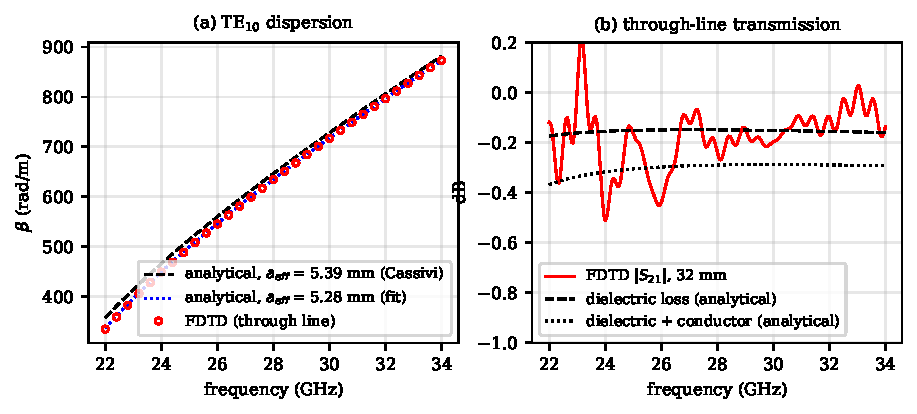
\includegraphics[width=\linewidth]{fig_validation}
\caption{Validation of the FDTD solver on an SIW through line: (a) TE$_{10}$ phase constant versus the analytical model; (b) transmission over 32~mm versus the analytical dielectric and conductor losses.}\label{fig:validation}\end{figure}

\section{Sub-array synthesis}\label{sec:design}
\subsection{Geometry}
The antenna (Fig.~\ref{fig:geometry}) consists of two parallel SIWs with centre spacing $D = \SI{7.0}{mm}$ ($0.65\lambda_0$), each carrying five longitudinal slots of width $w = \SI{0.4}{mm}$, alternately offset by $\pm x_0$ from the SIW axis, spaced by $d_s = \lambda_g/2$ and terminated by a shorting via wall at $\lambda_g/4$ from the last slot, i.e. a standing-wave array \cite{elliott2003}. The two SIWs are fed at the opposite end (ports P1 and P2). The region between the inner via rows of the two SIWs is a \SI{1.4}{mm} wide dielectric channel, below cut-off at 28~GHz, covered by the common top metal in which the decoupling slits are etched. The total thickness is the substrate plus two copper layers, $\approx\SI{0.58}{mm}$ ($0.054\lambda_0$).

\begin{figure}[t]\centering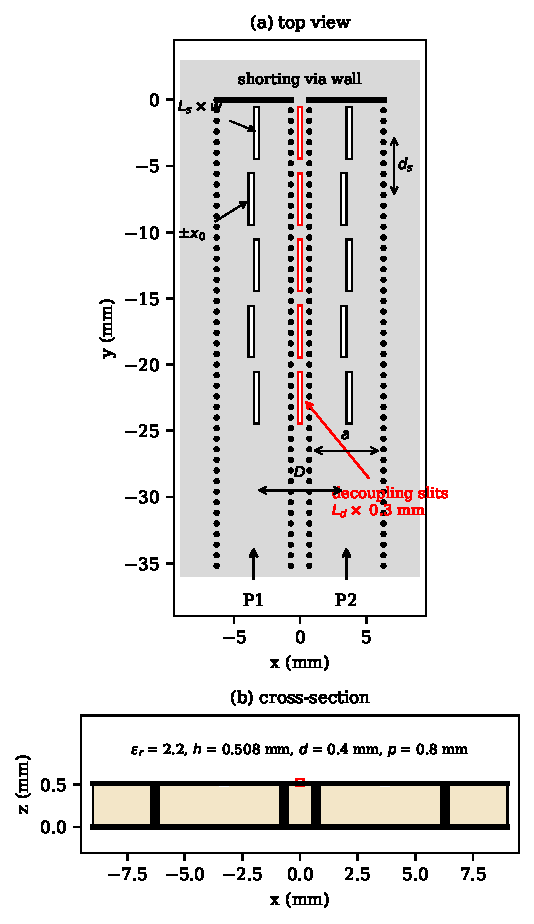
\includegraphics[width=\linewidth]{fig_geometry}
\caption{Dual-port SIW slot array with characteristic-mode-guided decoupling slits: (a) top view; (b) cross-section.}\label{fig:geometry}\end{figure}

\subsection{Single-slot characterisation}
Elliott's procedure requires the resonant length and the resonant conductance of an isolated slot as functions of its offset. Both were obtained with the FDTD solver from a single slot in a matched SIW through line: the shunt admittance normalised to the TE$_{10}$ characteristic admittance is $y = g + \mathrm{j}b = 2(1-S_{21})/S_{21}$, where $S_{21}$ is referred to the slot-free line. Fig.~\ref{fig:slot}(a) shows $y(f)$ for $x_0 = \SI{0.2}{mm}$ and several lengths, Fig.~\ref{fig:slot}(b) the resonant frequency ($b = 0$) versus length for three offsets and Fig.~\ref{fig:slot}(c) the resonant conductance versus offset. Two features distinguish the thin SIW from the classical thick waveguide. First, the resonant conductance is very large: the least-squares fit $g_r = K\sin^2(\pi x_0/a)$ gives $K = \Kfit$, whereas the Stegen formula $g_r = 2.09(a/b)(\lambda_g/\lambda_0)\cos^2(\pi\lambda_0/2\lambda_g)\sin^2(\pi x_0/a)$ \cite{elliott2003} with $b = h$ gives $K \approx 0.5$, because its $\cos^2$ factor is derived for $\lambda_g > \lambda_0$ and is not applicable to the dielectric-filled guide where $\lambda_g < \lambda_0$. Second, the resonant frequency depends strongly on the offset (\SI{27.9}{GHz} at $x_0 = \SI{0.5}{mm}$ but \SI{26.4}{GHz} at $x_0 = \SI{0.2}{mm}$ for $L_s = \SI{4.5}{mm}$), because the internal reactive loading by the guide is comparable to the external slot reactance. Consequently the slot data must be taken at the offset actually used. At $x_0 = \SI{0.2}{mm}$ the interpolated 28~GHz resonant length of the isolated slot is \LresIso~mm and $g_r \approx \gslot$. (Slot lengths are quoted in the on-grid convention of the FDTD model: aperture edges on grid lines with the edge nodes metallic, so that the length resolution is \SI{0.2}{mm}.)

\begin{figure}[t]\centering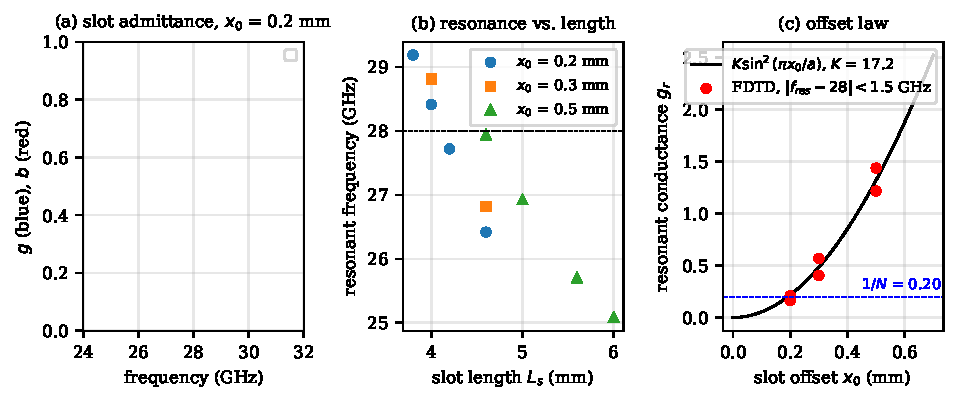
\includegraphics[width=\linewidth]{fig_slot}
\caption{Full-wave characterisation of a longitudinal slot in the \SI{0.508}{mm} SIW: (a) normalised admittance for $x_0 = \SI{0.2}{mm}$; (b) resonant frequency versus slot length; (c) resonant conductance versus offset with the $\sin^2$ fit; the dashed line is the conductance $1/N$ required for a matched $N$-slot standing-wave array.}\label{fig:slot}\end{figure}

\subsection{Elliott synthesis}
For a uniform standing-wave array the slot conductances are $g_n = 1/N$ so that the input is matched ($\sum g_n = 1$) \cite{elliott1983,elliott2003}. With $K = \Kfit$, $g_n = 0.2$ requires $x_0 = \SI{0.19}{mm}$; the offset is rounded to the \SI{0.2}{mm} grid of the FDTD model ($\sum g_n = \gsum$, i.e. $|S_{11}| \approx \SSum$ at resonance). A five-slot sub-array is therefore the natural choice for this substrate: a four-slot array would need $g_n = 0.25$ and an offset of \SI{0.22}{mm}, while the larger offsets of a conventional design would over-couple the slots. The slot spacing $d_s = \lambda_g/2 = \SI{4.96}{mm}$ and the distance from the short, $\lambda_g/4 = \SI{2.48}{mm}$, were rounded to \SI{5.0}{mm} and \SI{2.5}{mm}. The first full-wave run of the complete array with the on-grid length $L_s = \SI{4.0}{mm}$ showed the band centred at \SI{27.5}{GHz}, because the external mutual coupling between the five slots lowers their resonance by about \SI{0.9}{GHz} with respect to the isolated slot; a single iteration with the next shorter on-grid length, $L_s = \Lres$~mm, centres the band at \fcDec~GHz (Section~\ref{sec:results}). This two-step flow, first-order Elliott synthesis followed by one full-wave correction, replaces the iterative second-order procedure of \cite{elliott1983} at a cost of one array simulation.

\section{Characteristic-mode-guided decoupling}\label{sec:cma}
\subsection{Coupling mechanism}
With the sub-arrays driven separately, the slots of the two SIWs are parallel and displaced in the E-plane of the slots (the $x$-direction), which is the strongest-coupling configuration for slots in a common ground plane. Since the region between the SIWs is a below-cut-off channel, the coupling is carried exclusively by the exterior: by the space wave and by the surface current that flows across the \SI{1.4}{mm} wide strip of top metal between the inner via rows. The FDTD result without any decoupling structure (Section~\ref{sec:results}) gives $|S_{21}| = \IsoRefTwentyEight$~dB at 28~GHz.

\subsection{Aperture-mode design of the slits}
A resonant slit of length $L_d$ etched in the top wall along $y$ presents, at its characteristic resonance, a high impedance to the $x$-directed surface current and acts as a parasitic aperture whose scattered field cancels part of the direct coupling. The slit is modelled in the magnetic-current formulation (\ref{eq:ymn}) as an aperture in an infinite ground plane with air above and an effective dielectric half-space below. The effective permittivity accounts for the thin grounded substrate under the aperture and is calibrated once from the full-wave data of Section~\ref{sec:design}: the isolated radiating slot that resonates at 28~GHz in the FDTD model ($L_s = \LresIso$~mm, $x_0 = \SI{0.2}{mm}$) has its aperture-mode resonance ($\alpha_1 = 180^\circ$) at \fAir~GHz in air and at 28~GHz for $\varepsilon_{\mathrm{eff}} = \epsEff$ (Fig.~\ref{fig:cmacal}(a)). With this medium the aperture-mode resonance of a \SI{0.3}{mm} wide slit is computed as a function of its length (Fig.~\ref{fig:cmacal}(b)); the length for a 28~GHz characteristic resonance is $L_d = \Ld$~mm, implemented as \Lduse~mm on the \SI{0.2}{mm} length grid of the FDTD model. Five such slits are centred on the axis $x = 0$ of the channel, one in front of each slot pair, so that the slit mode is excited by the transverse current of every slot.

\begin{figure}[t]\centering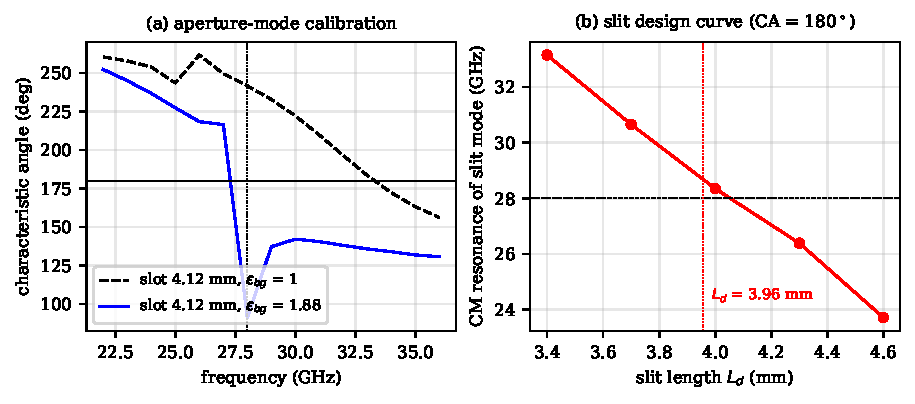
\includegraphics[width=\linewidth]{fig_cma_cal}
\caption{Aperture-mode (magnetic-current) characteristic-mode analysis: (a) characteristic angle of the dominant mode of the radiating slot in air and in the calibrated effective medium; (b) resonance of the decoupling slit versus its length.}\label{fig:cmacal}\end{figure}

\subsection{Characteristic modes of the shared top wall}
The effect of the slits on the modes of the shared conductor is examined with the electric-current formulation (\ref{eq:zmn}) applied to the top wall of the two sub-arrays (\platesize, ten slots, with and without the five slits of \Lduse~mm, background permittivity $\varepsilon_{\mathrm{eff}}$). For every mode a gap-crossing index
\begin{equation}
\mathrm{GCI}_n = \frac{\int_{\mathrm{gap}} |J_{x,n}|\,\mathrm{d}S}{\int_{\mathrm{plate}} |\mathbf{J}_n|\,\mathrm{d}S}
\end{equation}
measures the fraction of its current that crosses the channel between the inner via rows in the $x$-direction, i.e. its ability to carry energy from one sub-array to the other. Fig.~\ref{fig:cmams} shows the modal significance of the modes with the largest GCI at 28~GHz without and with slits, and Fig.~\ref{fig:cmacur} the eigencurrent of the strongest gap-crossing mode in both cases. Without slits the coupling mode has $\mathrm{MS} = \MSref$ and $\mathrm{GCI} = \GCIref$ at 28~GHz: its current flows transversely across the gap between the slots of the two sub-arrays. With the slits the current of the same family of modes is forced to circulate around the slits, and the largest GCI of any significant mode at 28~GHz drops to \GCIslit; the slit mode itself appears as a mode with current concentrated along the slit edges. This modal picture is the design criterion: the slit length is chosen such that the slit mode is resonant at the centre frequency, which maximises the perturbation of the gap-crossing current.

\begin{figure}[t]\centering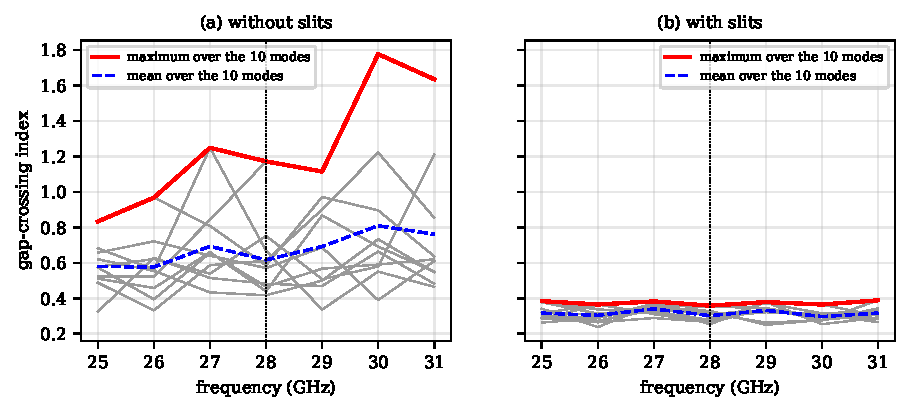
\includegraphics[width=\linewidth]{fig_cma_ms}
\caption{Modal significance of the characteristic modes of the shared top wall with the largest gap-crossing index (GCI at 28~GHz in the legend): (a) without and (b) with the decoupling slits.}\label{fig:cmams}\end{figure}

\begin{figure}[t]\centering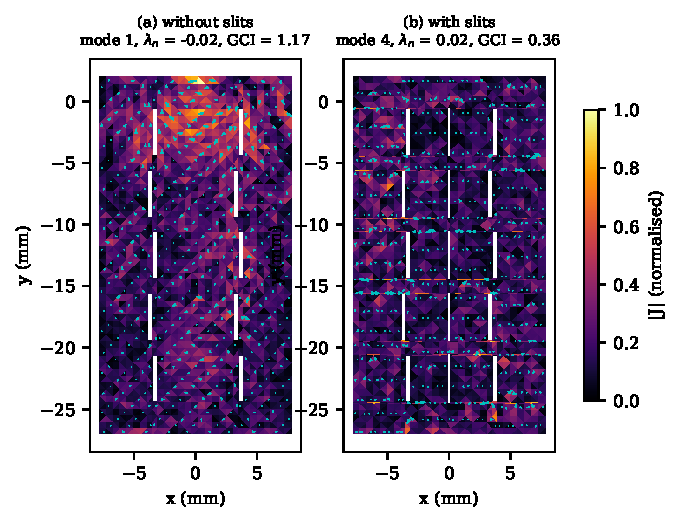
\includegraphics[width=0.8\linewidth]{fig_cma_currents}
\caption{Eigencurrent of the characteristic mode with the largest gap-crossing index at 28~GHz: (a) without and (b) with the decoupling slits (colour: $|\mathbf{J}_n|$, arrows: real part).}\label{fig:cmacur}\end{figure}

\section{Full-wave results and discussion}\label{sec:results}
\subsection{S-parameters}
Fig.~\ref{fig:sparams} shows the FDTD reflection and transmission coefficients of the final array ($L_s = \Lres$~mm) without slits and with the CMA-dimensioned slits ($L_d = \Lduse$~mm), and Table~\ref{tab:sweep} the effect of the slit length. Without slits the $-10$~dB band is \BWref~GHz (\BWrefRel\,\%) and the isolation is \IsoRefTwentyEight~dB at 28~GHz with a minimum of \IsoRefMin~dB in the band. The slits improve the isolation to \IsoDecTwentyEight~dB at 28~GHz and to a minimum of \IsoDecMin~dB over the common band \BWdec~GHz, i.e. by \IsoGain~dB at the centre frequency, while the reflection coefficient remains below $-10$~dB over \BWdecRel\,\%. The slit-length sweep confirms that the CMA prediction is close to the full-wave optimum: \SweepSentence. The decoupling mechanism is therefore the characteristic resonance of the slits, not a mere interruption of the metal, and the aperture-mode CMA with a single calibration constant predicts the required length to within the \SI{0.1}{mm} resolution of the model.

\begin{figure}[t]\centering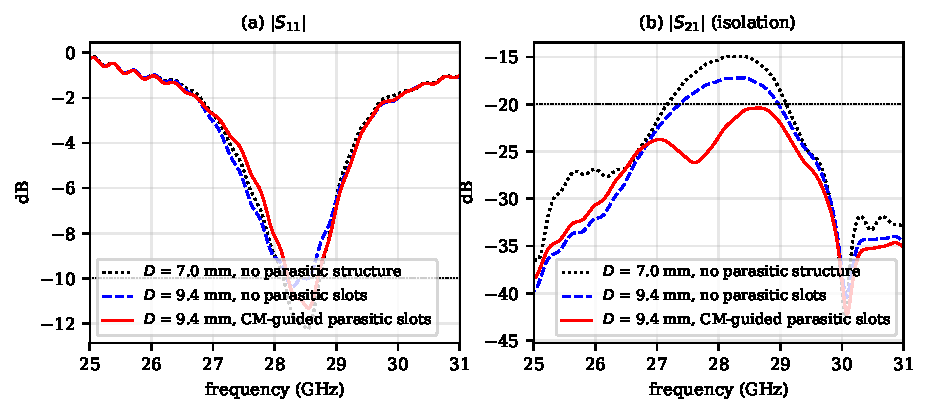
\includegraphics[width=\linewidth]{fig_sparams}
\caption{FDTD S-parameters of the dual-port array without and with the CM-guided slits: (a) reflection; (b) isolation.}\label{fig:sparams}\end{figure}

\begin{table}[t]\centering\caption{Effect of the slit length (FDTD, port 1 excited).}\label{tab:sweep}
\small\begin{tabular}{cc}\toprule a & b\\\midrule 1 & 2\\\bottomrule\end{tabular}
\end{table}

\subsection{Radiation}
Fig.~\ref{fig:radiation} shows the embedded gain patterns of port 1 at 28~GHz in the two principal planes, the realised gain versus frequency and the ECC computed from the embedded patterns. The sub-array radiates a broadside beam with a realised gain of \GainDec~dBi at 28~GHz with the slits (\GainRef~dBi without), a half-power beamwidth of about \HPBWe$^\circ$ in the $y$-$z$ plane (five slots) and \HPBWh$^\circ$ in the $x$-$z$ plane (single SIW width), and a radiation efficiency of \EffDec\,\% (dielectric loss only; the copper is modelled as PEC, so that the conductor loss of about \CondLoss~dB estimated analytically for the \SI{25}{mm} slot section should be subtracted from the realised gain). Without slits the strong coupling tilts the beam of the excited sub-array by \TiltRef$^\circ$ towards the parasitic sub-array in the $x$-$z$ plane; with the slits the tilt is reduced to \TiltDec$^\circ$. The ECC between the two ports drops from \ECCref to \ECCdec at 28~GHz. The slits radiate a small cross-polarised component which is included in the patterns and in the efficiency.

\begin{figure}[t]\centering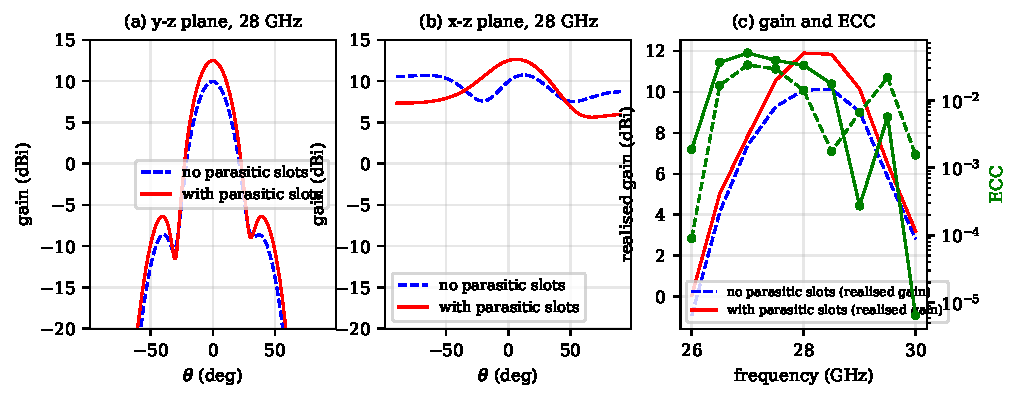
\includegraphics[width=\linewidth]{fig_radiation}
\caption{FDTD radiation results for port 1: (a) $y$-$z$ plane and (b) $x$-$z$ plane gain patterns at 28~GHz; (c) realised gain and ECC versus frequency.}\label{fig:radiation}\end{figure}

\subsection{Comparison with the literature}
Table~\ref{tab:comp} compares the proposed antenna with reported 28~GHz SIW slot arrays and decoupled mmWave arrays. The proposed design combines the lowest profile with an isolation that is comparable to that of dedicated decoupling networks \cite{diman2021} or shields \cite{alibakhshikenari2019,dey2021}, while using no additional layer, component or footprint. Its bandwidth is that of a standing-wave array; a travelling-wave or centre-fed configuration would widen it at the cost of a frequency-scanning beam, which is left for future work.

\begin{table}[t]\centering\caption{Comparison with reported mmWave SIW slot arrays and decoupled arrays (simulated results of this work).}\label{tab:comp}
\small\begin{tabular}{@{}lccccc@{}}\toprule
Ref. & $f_0$ (GHz) & Profile ($\lambda_0$) & Gain (dBi) & Isolation (dB) & Decoupling \\\midrule
\cite{ashraf2015} & 28/38 & 0.047 & 11.9 & -- & -- (single port)\\
\cite{lai2020} & 28/38 & 0.05 & 9.3--10.9 & -- & -- (single port)\\
\cite{singh2021} & 28 & 0.05 & 12.3 & -- & -- (single port)\\
\cite{kobal2022} & 28 & 0.07 & 4.7/8 & $>30$ & port placement (annular slot)\\
\cite{diman2021} & 10 & 0.05 & -- & 35 & two-layer SIW coupler network\\
\cite{alibakhshikenari2019} & 60 & 0.15 & 10.1 & $\approx 25$ & metamaterial shield\\
\cite{dey2021} & 28 & $>0.1$ & 9--13.3 & $>40$ & stacked EBG + DGS\\
This work & 28 & 0.054 & \GainDec & \IsoDecMin--\IsoDecTwentyEight & CM-guided slits in top wall\\
\bottomrule\end{tabular}\end{table}

\subsection{Limitations}
The results are numerical. The FDTD model uses PEC metal, an infinite ground plane and a \SI{0.1}{mm} staircase grid; the via representation shifts $a_{\mathrm{eff}}$ by \aeffDiff\,\%, which was compensated by using the full-wave $\lambda_g$ in the synthesis. The aperture-mode CMA uses a single effective permittivity calibrated from one full-wave slot resonance; it predicted the slit length to within the \SI{0.2}{mm} length resolution of the model, but the final value should always be confirmed by a short full-wave sweep, as done here. A microstrip-to-SIW transition and a measurement on a fabricated prototype are the natural next steps; the released environment allows both to be simulated without proprietary software.

\section{Conclusion}\label{sec:concl}
A dual-port, low-profile SIW slot array for 28~GHz 5G front ends has been designed entirely with an open-source hybrid FDTD/MoM environment developed for this work, and its port isolation has been improved by \IsoGain~dB at 28~GHz with resonant slits in the shared top wall whose length was obtained from a characteristic-mode analysis of the aperture system and verified on the finite top wall through the gap-crossing current of the coupling mode. The design flow, from the SIW equations through the full-wave slot characterisation, the Elliott synthesis, the CMA-based slit dimensioning and the full-wave verification, is reproducible from the released scripts. The same environment and method apply directly to larger tiles (more sub-arrays side by side), to dual-polarised SIW arrays and to other mmWave bands.

\section*{Declaration of competing interest}
The author declares no competing financial interests or personal relationships that could have influenced the work reported in this paper.

\section*{Data availability}
The complete source code of the design environment, all scripts and all simulation data are available in the repository accompanying this article.

\bibliographystyle{elsarticle-num}
\bibliography{refs}
\end{document}
